\section{Global Cube Welding}
\label{sec:weld}

\plain{In brief: cubes are meshed independently, so the natural next step is to sew their sheets back together across the cube faces. ScrollFiesta can do this, and the result is instructive --- but the active whole-sheet path deliberately does not require it, for a reason worth stating carefully.}

Welding is optional in the current system, and understanding why is more useful than the weld itself. A geometric weld makes an assertion of the strongest possible kind: these two triangles are the same surface. Once made, that assertion is indistinguishable from a triangle that was measured, and by Section~\ref{sec:gp} no downstream geometric test can question it. Meanwhile, per-cube reconstruction and remeshing can leave divergent seam triangulations even where the halo voxels agree, so the weld is being asked to make a hard topological claim on the basis of a soft geometric coincidence. The ribbon fit of Section~\ref{sec:quadribbon} can instead close cube seams from material claims, treating continuity as a \emph{fitted relation} that carries its own confidence. The active path therefore consumes the pre-weld pile.

We retain the weld for three reasons: local welding is genuinely useful for verified patches; the welder is used as a sub-engine by the unwrapper to ask whether two sheets adjacent in $(u,v)$ are actually neighbours in the scroll; and it is the correct frozen yardstick for upstream A/B comparisons and for comparison with earlier published results.

\subsection{Seam-Band Reconstruction}

We first place every accepted cube mesh in volume coordinates and concatenate it under the ownership established by halo trimming. The uniformly coarse CVT interiors are desirable for scale, but their triangles are too large for the weld's ball --- radius at most three voxels --- to initialize reliably. We therefore detect every internal cube plane and refine only a narrow seam band to approximately 3.5-voxel triangles (Fig.~\ref{fig:weld_bands}). Boundary half-edges in that band seed the same BPA used per cube, and four sub-processes then connect matching fronts while rejecting invalid joins.

A \textbf{sliver cull} first removes near-degenerate boundary triangles that would prime the bridge ball off a needle. The \textbf{bridge front} escalates its radius adaptively from the local boundary spacing, capped so that twice the maximum radius stays below the measured ${\sim}7$-voxel inter-wrap clearance: welding two wraps together is thereby made geometrically impossible for the bridge, rather than merely penalized. This is a deliberate design choice --- where a physical constant of the object is available, we prefer to make the failure unreachable rather than expensive.

Every candidate bridge face must additionally pass a \textbf{winding test}. Using the winding coordinate of Equation~\eqref{eq:winding}, the phase gap $w$ between front and candidate must stay within a soft tolerance of 0.35 turns, with a 0.40-turn hard cap that separates legitimate grazing-seam closures from cross-layer and next-wrap stitches. The same test is what keeps recto from welding to verso. Finally, a \textbf{sheet-correspondence pass} recovers legitimate same-sheet closures that the conservative test rejected: it confirms a mutual-best one-to-one sheet pairing across each seam from bridge votes and boundary overlap, then re-welds only that confirmed pair, on a point cloud restricted to those two sheets.

\subsection{Recoarsening Under Invariants}

After each weld the temporary fine band is recoarsened and optimized with a \emph{pinned-boundary} CVT/RVD pass. Boundary positions are held bit-exact while interior sites solve the same centroidal and normal-anisotropy objective as Section~\ref{sec:cvt}. A proposed band patch is accepted only if every pin is represented, the complete boundary-edge set is unchanged, all edges remain manifold, and both component count and Euler characteristic equal their pre-remesh values. Tiled passes with an offset allow long seams to be processed at bounded memory, and if any invariant fails, that tile simply retains the pre-CVT weld. The pattern here recurs throughout the system: an optimization is allowed to improve a representation only when it can prove it did not change what the representation means.

\subsection{Checking the Result}

Orientation consistency alone is insufficient to guarantee a valid scroll: a perfectly manifold bridge may still connect turns that are far apart in scroll phase. The global scan therefore measures abrupt full-turn edges \emph{and} computes a branch-local phase span, which is what detects broad fusions assembled from individually plausible edges. A phase sever can remove faces crossing those discontinuities, but its output is not relied on until every resulting component also satisfies the broad-span test.

\begin{figure}[t]
  \centering
  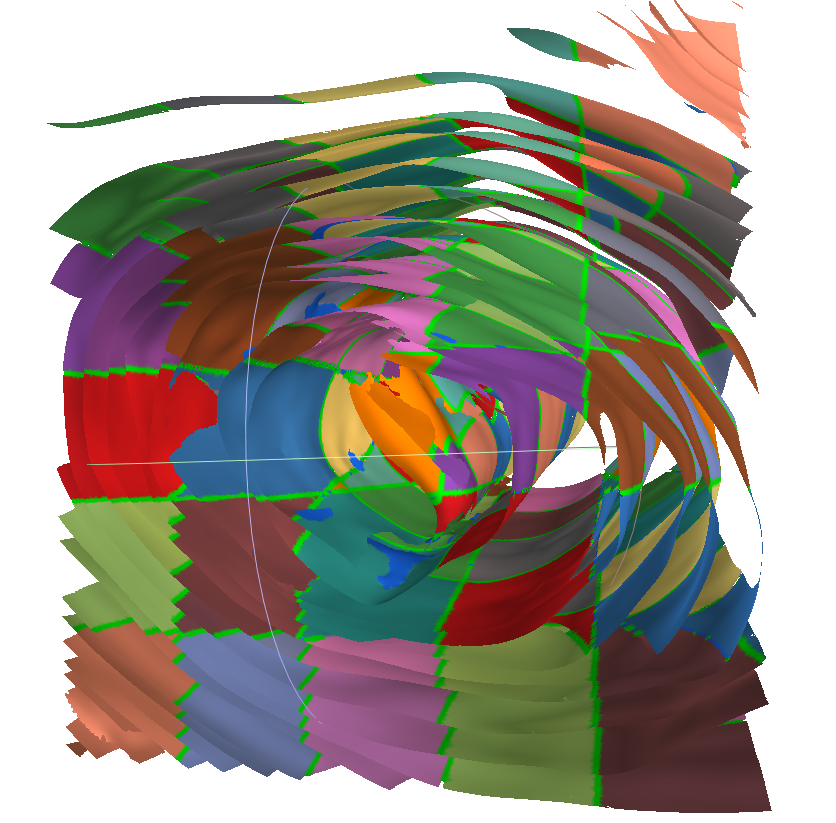
\includegraphics[width=\linewidth]{figures/welded_cube_4x5x5.png}
  \caption{The welded $4\times5\times5$ block with each cube's sheet coloured independently and the refined seam bands drawn in green. The weld bridges the ${\sim}$1-voxel trim gap between adjacent cubes only inside these bands; the winding test and the capped bridge radius decide which fronts may join, so a sheet continues across a seam exactly when the two cubes agree it is the same wrap.}
  \Description{A rendered stack of curved papyrus sheets divided into cube-sized coloured tiles, with thin green bands marking the welded cube boundaries.}
  \label{fig:weld_bands}
\end{figure}

The weld is designed to compose hierarchically: a group of placed cubes, or of previously welded blocks, enters the same seam-band procedure. The complete demonstration is a flat $4\times5\times5$ block; the long $4\times21\times21$ experiment is decomposed into axial strips at the atlas level, while the fully hierarchical geometry weld remains active work.
